% \section{Example problem: homogeneous block model}
% \label{example}

% \subsection{Preliminary considerations}
% To illustrate the usage of \texttt{SOFI2D}, we use a homogeneous block model. The material parameters of the block are: P-wave velocity $V_P=\SI{3369}{m/s}$, S-wave velocity $V_S=\SI{1643}{m/s}$ and density $\rho=\SI{2000}{kg/m^3}$. A point-force source in the vertical direction is located inside the model at point $x_s=\SI{398}{m}$ and $y_s=\SI{398}{m}$}. The source function is a Ricker wavelet (see Chapter \ref{sources}) with a center frequency $f_c=\SI{5}{Hz}$. To calculate the dimensions of the grid the spatial grid spacing is estimated using the grid dispersion criterion. \textcolor{red}{For a 4th order Holberg FD operator using $V_{S,min}=\SI{1643}{m/s}$, $f_{max}=2 \cdot f_c=\SI{10}{Hz}$ and $n=...$ we get:}
% \begin{equation}
%     \Delta h \le \frac{V_{s,min}}{n\; f_{max}} = ...\;\mathrm{m}\;.
% \end{equation}
% \textcolor{red}{The whole model grid has the dimensions 400 x 400 gridpoints}. To avoid a violation of the Courant criterion the time step size $\Delta t$ is calculated according to using $V_{P,min}=\SI{3369}{m/s}$, $h=1.0$ and $\Delta h=\SI{0}{m}$:
% \begin{equation}
%     \Delta t \le \frac{\Delta h}{h \sqrt{2} v_{p,max}} = ... \times 10^{-3} s \approx ...\; \mathrm{ms}\;.
% \end{equation}
% \textcolor{red}{The modeling covers a time span of \SI{5.0}{s}, so about $NT=$ 649 time steps are needed. A line of 100 geophones is placed between $x_{start}=\SI{54}{m}$ and $x_{end}=\SI{5400}{m}$ and a constant depth of $y=\SI{2106}{m}$.} 

% \textcolor{red}{Attenuation parameters: $Q_P=Q_S=\SI{8}{}$.}

% \textcolor{red}{Anisotropic parameters: $\epsilon=\SI{0.26}{}$, $\delta=\SI{-0.05}{}$, $\theta=\SI{30}{}$.}

\section{Definition of the modeling parameters}
\label{modelgeom}
The geometry of the FD grid and all parameters for the wavefield simulation have to be defined in a parameter file (which we name in this case \texttt{sofi2D.json}). In the following we will explain all input parameters in detail.
%%\input{sofi2D.json}
All lines in the parameter file are formated according to the JSON standard~(\url{http://www.json.org}) and organized as 
\begin{verbatim}
"VARNAME" = "Parameter value",
\end{verbatim}
where a comment line can look like this:
\begin{verbatim}
"Comment" = "This is a useful comment",
"3D Grid information" = "comment",
\end{verbatim}
Here, \texttt{VARNAME} is a symbolic name for the actual different parameters shown below. Basically, all non-JSON conforming lines will be ignored. The order of the various parameters does not matter, but we typically group parameters that belong together. If critical parameters are missing, the code will stop and an error message will appear. The program outputs the read and all updated/adjusted and possibly calculated parameters unless such output is suppressed.

\subsection{Domain decomposition}
\begin{verbatim}
"Domain Decomposition" : "comment",
            "NPROCX" : "4",
            "NPROCY" : "2",
\end{verbatim}

with

\texttt{NPROCX} : number of (MPI) processors in x-direction\\
\texttt{NPROCY} : number of (MPI) processors in y-direction

\begin{figure}[ht!]
\centering
    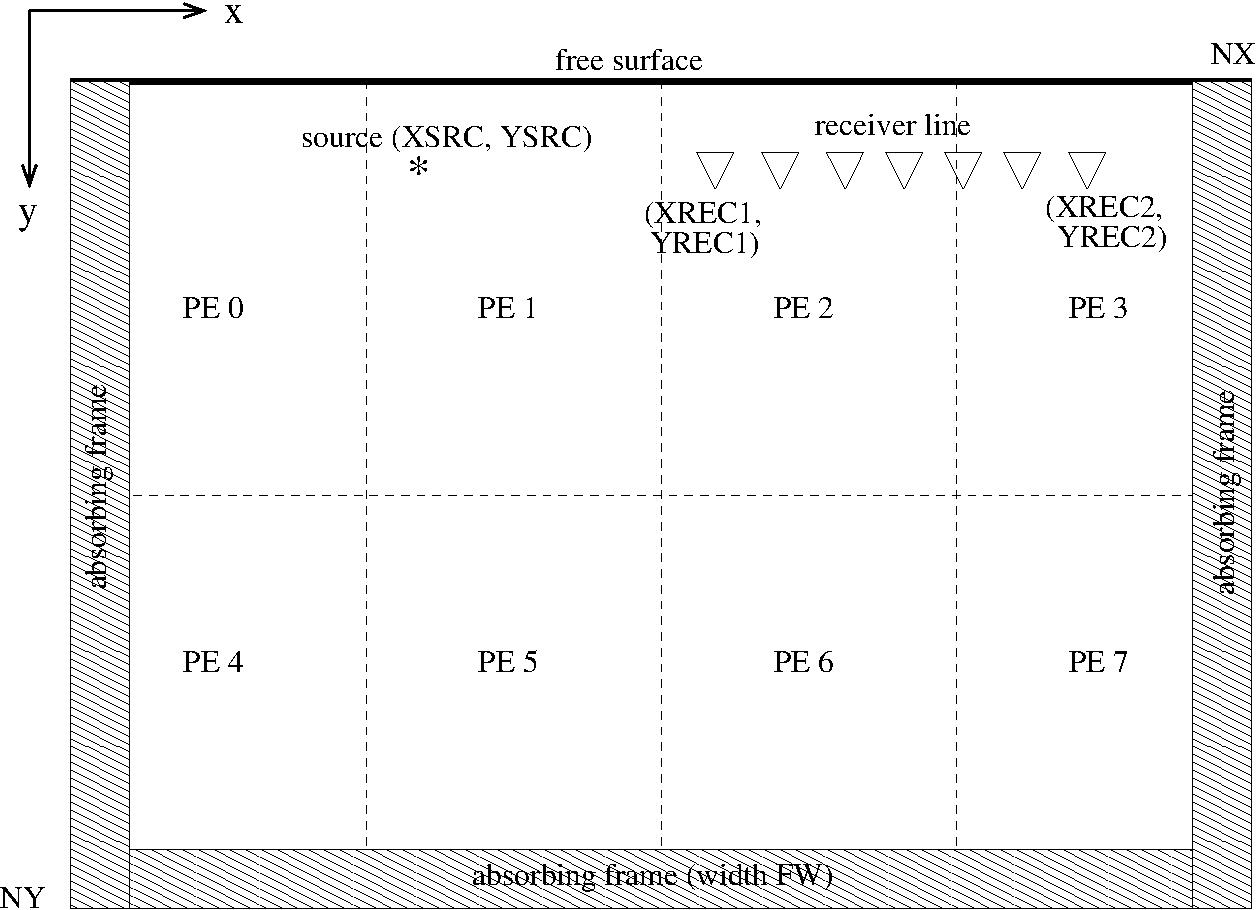
\includegraphics[width=12cm,angle=0]{figures/grid.pdf}
    \caption{Geometry of the numerical FD grid using 4 processors in the $x$-direction (\texttt{NPROCX=4}) and 2 processors in the $y$-direction (\texttt{NPROCY=2}). At the top of the numerical mesh, the PEs apply a free surface boundary condition if \texttt{FREE\_SURF}=1, otherwise an absorbing boundary condition is used; the width of the absorbing frame is \texttt{(FW-1)*DH} in meters. The size of the total grid is \texttt{NX} grid points in the $x$-direction and \texttt{NY} gridpoints in the $y$-direction. The origin of the Cartesian coordinate system is at the top left corner of the grid, i.e., the first upper-left grid point corresponds to coordinate $x=0$, $y=0$.}
\label{fig_grid}
\end{figure}

Parallelization is based on domain decomposition (see Fig.~\ref{fig_grid}), i.e., each processing element (PE) updates the wavefield within its portion of the grid. The model is decomposed by the program into subgrids (blocks). After decomposition, each processing elements (PE) saves only its sub-volume of the grid. \texttt{NPROCX} and \texttt{NPROCY} specify the number of (MPI) processors in horizontal and vertical direction, respectively (Fig.~\ref{fig_grid}). Thus, the total number of processors is \texttt{NP=NPROCX*NPROCY}; this values must be specified when starting the program with the following command: \texttt{mpirun -np $<$NP$>$ ../bin/sofi2D sofi2D.json}. If the total number of processors in \texttt{sofi2D.json} and the number of MPI processes differ, the program will terminate immediately with a corresponding error message. Obviously, the total number of PEs (\texttt{NPROCX*NPROCY}) used to decompose the model should be less or equal the total number of CPU cores available on your parallel processing machines or cluster. You can oversubscribe compute nodes but this usually hurts performance. In order to reduce the amount of data transferred between PEs, one should try to realize more or less cubic subgrids. In our example, we use 4 PEs in horizontal direction (\texttt{NPROCX=4}) and 2 PEs in vertical direction (\texttt{NPROCY=2}). The total number of PEs used by the program, and hence the number of MPI processes, is \texttt{NP=NPROCX*NPROCY=8}.

\subsection{Order of the FD operator}
\begin{verbatim}
"FD order" : "comment",
            "FDORDER" : "4",
            "FDORDER_TIME" : "2",
            "MAXRELERROR" : "1",
\end{verbatim}

with

\texttt{FDORDER} : order of the spatial FD operator (2, 4, 6, 8, 10 or 12)\\
\texttt{FDORDER\_TIME} : order of the temporal FD operator (2 or 4)\\
\texttt{MAXRELERROR} : Maximum relative group velocity error (Taylor=0; Holberg=1)

\texttt{FDORDER\_TIME}=2 correspondents to the classical leapfrog scheme and \texttt{FDORDER\_TIME}=4 to a fourth order accurate scheme. By the option \texttt{MAXRELERROR}, you can switch between Taylor and Holberg FD coefficients but also define a maximum of tolerated group velocity error in percent (Taylor coefficients=0, Holberg coefficients: 1 for $E=0.1\%$, 2 for $E=0.5\%$, 3 for $E=1.0\%$, and 4 for $E=3.0\%$). The chosen FD operator and FD coefficients have an influence on the numerical stability and grid dispersion (see next section).

\subsection{Space discretization}
\begin{verbatim}
"2-D Grid" : "comment",
            "NX" : "400",
            "NY" : "400",
            "DH" : "2.0",
\end{verbatim}

with

\texttt{NX} : number of grid points in the $x$-direction \\
\texttt{NY} : number of grid points in the $y$-direction\\
\texttt{DH} : distance between grid points in both spatial directions (grid size in meters)

These lines specify the size of the total grid (Fig.~\ref{fig_grid}) and therefore the size of external models. An equidistant grid is used in the FD software. The size of the total grid in $x$-direction is \texttt{(NX-1)*DH} and in $y$-direction \texttt{(NY-1)*DH}. \textbf{Note that the $y$-direction always corresponds to the vertical direction} (i.e., to depth). \texttt{NX/NPROCX} and \texttt{NY/NPROCY} must be integer values (for the time being, i.e., subdomains must have equal sizes -- this will be changed in a future version of the program).

To avoid numerical dispersion, the wavefield must be discretized with a certain number of grid points per wavelength. The number of grid points per wavelength depends on the order of the spatial FD operators used in the simulation. The criterion to avoid numerical dispersion is shown in eq.~\ref{eq:dh}; the program assumes that the maximum frequency of the source signal is approximately two times the center frequency. To avoid numerical dispersion of body waves, 8 grid points per minimum wavelength ($N=8$) are necessary for a fourth order algorithm and $N=12$ grid points for a second order algorithm (Table~\ref{grid_disp.2}. The dispersion criterion is checked by the FD software. See the SOFI2D log for further information or warnings. Please note that the FD code will not terminate due to grid dispersion.

\subsection{Time stepping}
\begin{verbatim}
"Time Stepping" : "comment",
			"TIME" : "0.5",
			"DT" : "1.0e-4",
\end{verbatim}

with

\texttt{TIME} : propagation time of seismic waves in the entire model (in seconds)\\
\texttt{DT} : time stepping interval (in seconds)

The time stepping interval $DT$ has to fulfill the stability criterion in eq.~\ref{courant_crit}, which is checked for the entire model. If the criterion is violated, the FD program will terminate with a corresponding error message. The maximum value for $DT$ at the stability limit is output, so you may simply try a certain $DT$, start the program, and then check what the program suggests as time step interval.

\subsection{Wave equations}
The parameter \texttt{WEQ} specifies the type of wave equation to use for modelling. Example:
\begin{verbatim}
"Wave Equation" : "comment",
            "WEQ" : "VEL_TTI",
\end{verbatim}
This parameter is given as string and can have the following values:
\begin{itemize}
\item \textbf{AC\_ISO}: acoustic isotropic wave equation
\item \textbf{VAC\_ISO}: viscoacoustic isotropic wave equation
\item \textbf{EL\_ISO}: elastic isotropic wave equation
\item \textbf{EL\_VTI}: elastic VTI wave equation
\item \textbf{EL\_TTI}: elastic TTI wave equation
\item \textbf{VEL\_ISO}: viscoelastic isotropic wave equation
\item \textbf{VEL\_VTI}: viscoelastic VTI wave equation
\item \textbf{VEL\_TTI}: viscoelastic TTI ave equation
\end{itemize}
The type of wave equation specified for \texttt{WEQ} determines which model files are read from disk and whether Q-related parameters are required, etc. Note that at the time of writing this manual not all wave equations have been implemented yet.

\subsection{Sources}
\label{sources}
\begin{verbatim}
"Source" : "comment",
            "SOURCE_SHAPE" : "1",
            "SIGNAL_FILE" : "signal_mseis.tz",
            "SIGOUT" : "0",
            "SIGOUT_FILE" : "./sources/signal_out01",
            "SIGOUT_FORMAT" : "1",
            "SOURCE_TYPE" : "3",
            "SOURCE_TOPO" : "0",
            "SRCREC" : "1",
            "SOURCE_FILE" : "./sources/source.dat",
            "RUN_MULTIPLE_SHOTS" : "0",
            "PLANE_WAVE_DEPTH" : "2106.0",
            "PLANE_WAVE_ANGLE" : "0.0",
            "TS" : "0.2",
\end{verbatim}

with

\texttt{SOURCE\_SHAPE} : shape of source-signal (Ricker=1; Fuchs-M\"uller wavelet=2; from \texttt{SIGNAL\_FILE}=3; sin$^3$=4; Berlage=5; Klauder=6)\\
\texttt{SIGNAL\_FILE} : external signal file name\\
\texttt{TS} : duration of the source-signal (in seconds)

Five built-in wavelets for the seismic source are available. The corresponding time functions are defined in \texttt{src/wavelet.c}. You may modify the time functions in this file and recompile to include your own analytical wavelet or to modify the shape of the built-in wavelets.

\textbf{Ricker wavelet}:
\begin{equation}
    A_r(\tau)= \left(1-2\tau^2\right)\exp(- \tau^2) \quad \mbox{with} \quad \tau=\frac{\pi(t-1.5/f_c-t_d)}{1.0/f_c}\;. 
    \label{eq_ricker}
\end{equation}

\textbf{Fuchs-M\"uller wavelet}:
\begin{equation}
    A_{fm}(t) = \begin{dcases} \sin(2\pi(t-t_d)f_c)-0.5\sin(4\pi(t-t_d)f_c)\,, & t\in[t_d,t_d+1/fc] \\
                 0\,, & \text{otherwise} \end{dcases}\;.
    \label{eq_fm}
\end{equation}

$\mathbf{sin^3}$ \textbf{wavelet}:
\begin{equation}
    A_{s}(t)=\begin{cases} \frac{3}{4} \pi f_c \sin(\pi(t+t_d)f_c)^3\,, & t \in[t_d,t_d+1/fc]\\
           0\,, & \text{otherwise} \end{cases}\;.
\label{eq_s3}
\end{equation}

\textbf{Berlage wavelet} (after \cite{aldrige:90}):
\begin{equation}
    A_b(t)=(t-t_d)^n\,e^{-\alpha (t-t_d)} \cos(2 \pi f_c (t-t_d) + \phi_0)\;.
    \label{eq_berlage}
\end{equation}

\textbf{Klauder wavelet} (after \cite{neelima:18}):
\begin{equation}
\begin{split} A_k(\tau) &= \Re \left\{ \frac{\sin\left(\pi k(\tau-t_d)\,(t_\text{sweep}-\tau+t_d)\right)}{ \pi k (\tau-t_d) e^{2 \pi i f_c (\tau-t_d)} } \right\} \\
\mbox{with} \quad k &= \frac{f_\text{max}-f_\text{min}}{t_\text{sweep}}\;,\quad\tau = t-\frac{n_\text{twidth}}{f_c}\quad\text{and}\quad f_c=\frac{f_\text{max}+f_\text{min}}{2}.\end{split}
    \label{eq_klauder}
\end{equation}

In these equations $t$ denotes time and $f_c$ is the center frequency. It is specified in the \texttt{SOURCE\_FILE} either directly, or for the Klauder wavelet calculated as half of $f_\text{max}+f_\text{min}$. If parameters are not provided through an external \texttt{SOURCE\_FILE} (\texttt{SRCREC=2}), the center frequency is derived through $f_c=1/TS$. $t_d$ is a time delay which can be defined for each source position in SOURCE\_FILE. Variable time delays for different sources locations allow the simulation of passive acoustic emission. Note that the symmetric (zero-phase) Ricker and Klauder signals are always delayed by $1.5/f_c$ for Ricker, and a shift of $n_\text{twidth}/f_c$ for Klauder, where $n_\text{twidth}$ is half the width of the wavelet in center periods. The Klauder wavelet is tapered on the first and last \qty{20}{\percent} with a cosine taper function. This means that for these two cases the maximum amplitude is excited at the source location after one and a half or $n_\text{twidth}$ centre periods, respectively. All source wavelets and the corresponding amplitude spectra for a center frequency of $f_c=\qty{50}{\hertz}$ and a delay of $t_d=0$ are plotted in Fig.~\ref{fig_source_wavelets}. Note the delay of the Ricker and Klauder signal described above. The Fuchs-M\"uller wavelet has a slightly higher center frequency and covers a broader frequency range. The Klauder wavelet covers a frequency range of \qty{10}{\hertz} to \qty{90}{\hertz} and uses a sweep duration of \qty{7}{\second} and $n_\text{twidth}$ of 5 center periods. For the Berlage wavelet, the additional parameters were set to $n=1.5$, $\alpha=210$, and $\phi_0=\qty{-90}{\degree}$.

\begin{figure}
\centering
    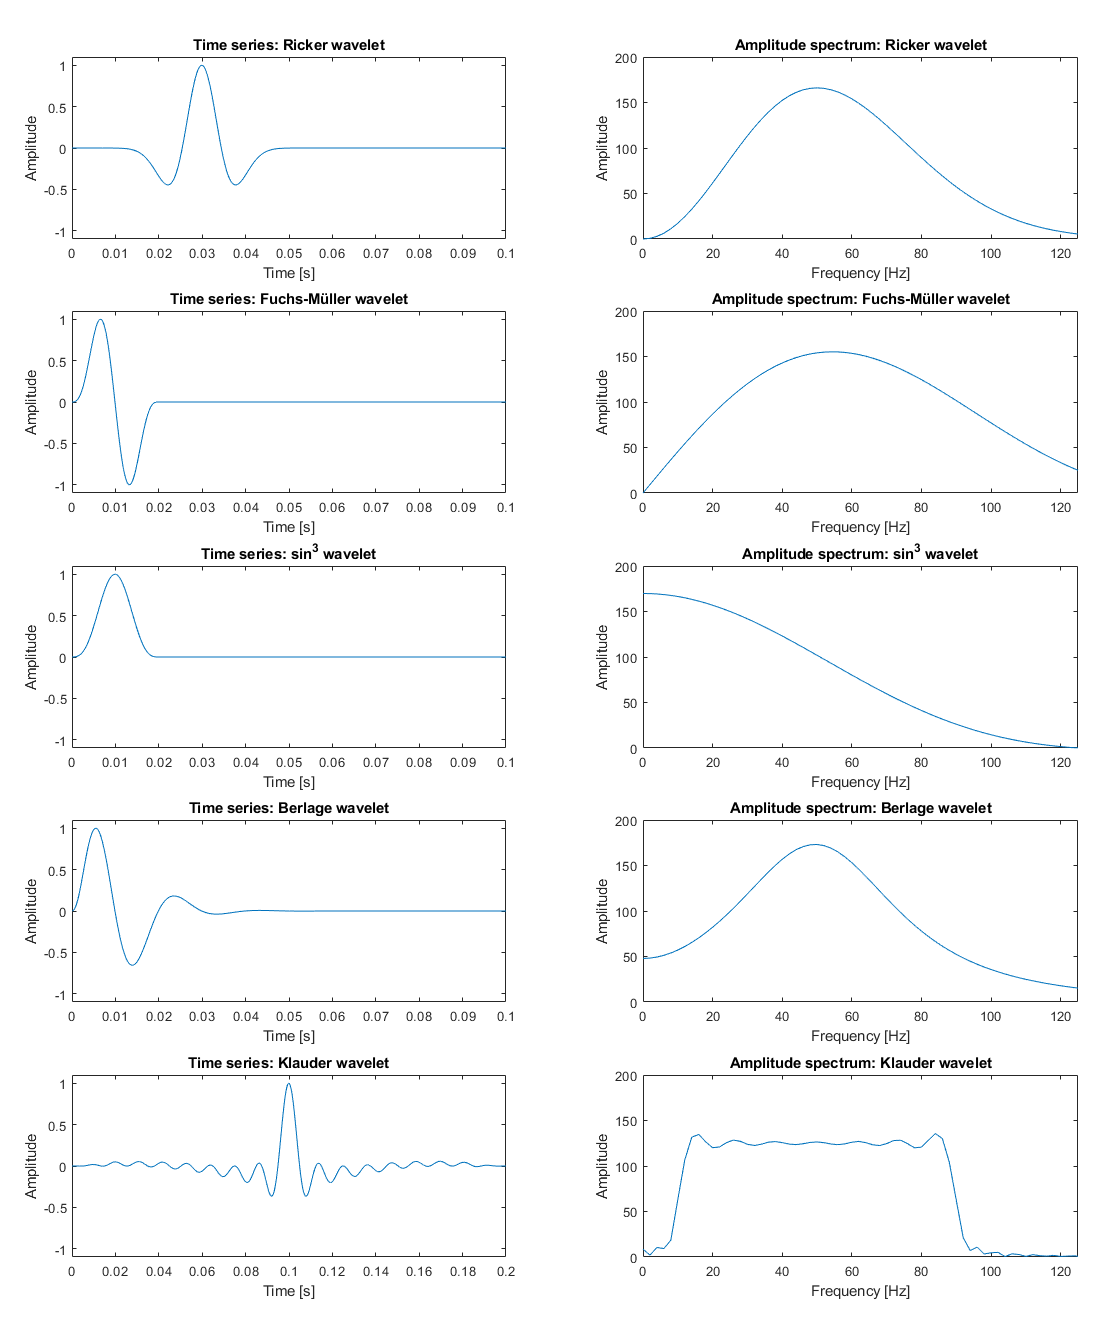
\includegraphics[width=0.9\textwidth]{figures/signals.png}
    \caption{Plot of built-in source wavelets for a center frequency of $f_c=\SI{50}{Hz}$ ($TS=1/f_c=\SI{0.02}{s}$): Ricker signal (1\textsuperscript{st} row), Fuchs-M\"uller signal (2\textsuperscript{nd} row), $sin^3$-signal (3\textsuperscript{rd} row), Berlage signal (4\textsuperscript{th} row), Klauder signal (5\textsuperscript{th} row). Time function (left column) and amplitude spectrum (right column).}
\label{fig_source_wavelets}
\end{figure}

You may also use your own digitized time function as the source wavelet (for instance the signal of the first arrival recorded by a geophone at near offsets). Specify \texttt{SOURCE\_SHAPE=3} and save the samples of your source wavelet in ASCII-format in \texttt{SIGNAL\_FILE}; this file should have a file suffix \texttt{.dat}, \texttt{.txt} or \texttt{.asc}. \texttt{SIGNAL\_FILE} should contain one sample (amplitude value) per line and have the following form:
\begin{verbatim}
# DT=0.0001
0.0
0.01
0.03
...
\end{verbatim}

The time interval between the samples must equal the time step interval (\texttt{DT}) of the FD simulation (see above)! It is therefore often necessary to resample/interpolate a given source time function with a smaller sample rate.

The ASCII file may contain a comment line in the beginning where the sampling interval can be specified as \texttt{DT=<value>} with the value being in seconds. This allows the program to cross-check that the FD time step interval matches the signature time sampling interval and the user does not accidentally modify \texttt{DT} in the parameter file without also updating the sampling interval of the source signature. If the aforementioned comment line is missing in the ASCII file, no cross-check is performed. In case of a mismatch, the program will abort.

The source signature can also be provided as SU-formatted file containing once trace (additional traces will be ignored). In this case, \texttt{SIGNAL\_FILE} should have the file suffix \texttt{.su}. Just like models in SU format, this file needs to use 32-bit native floats. The SU header \texttt{delrt} must be zero (signatures starting at non-zero times are not supported). The SU header \texttt{dt} (in microseconds), if given and greater than 0, is converted to seconds and then cross-checked against the FD time step interval. In case of a mismatch, the program will abort. Note that there is never an automatic interpolation performed by the program (neither when reading ASCII nor when reading SU files).

\texttt{SIGOUT} : output source wavelet (yes=1; no=0)\\
\texttt{SIGOUT\_FILE} : external signal file name for output\\
\texttt{SIGOUT\_FORMAT} : supported output formats (SU=1; ASCII=2; BINARY=3)

The wavelet can be output for quality control purpose by setting \texttt{SIGOUT} to 1 (default value is 0, i.e., no output). This works for both internally generated wavelets based on the parameters provided in \texttt{SOURCE\_FILE} and for externally provided wavelets read from \texttt{SIGNAL\_FILE}. In case QC output is requested, a basename for the output file has to be provided (\texttt{SIGOUT\_FILE}) and an output format (\texttt{SIGOUT\_FORMAT}).

\texttt{SOURCE\_TYPE} : source type (explosive=1; force in $x$-direction=2; force in $y$-direction=3; custom force=4)

\texttt{SOURCE\_TYPE=1} is equivalent to an explosive source that excites P-waves only radiating with the same amplitude into all directions. \texttt{SOURCE\_TYPE}=2 and \texttt{SOURCE\_TYPE}=3 simulate point forces in the $x$- and $y$-directions, respectively. With \texttt{SOURCE\_TYPE}=4, a source in a user-defined direction can be chosen which is defined by the parameter \texttt{SOURCE\_AZIMUTH} specified in in the \texttt{SOURCE\_FILE} (see Fig.~\ref{fig_source_azimuth}). These sources have specific radiation characteristics and excite both P- and S-waves. In case of an explosive source the diagonal components of the stress tensor are assigned with the source wavelet. In case of a directive force in the $x$- or $y$-directions, respectively, the corresponding external body force component ($f_i$, see Eq. 11 of \citep{bohlen:02} is assigned with the source wavelet amplitudes. Please not, that due to the 2D FD scheme, a point force is physically described as a line source. The excited wavefield is therefore not directly comparable to a 3D wave propagation. For 1D media, there is a 2D-to-3D conversion of both body and surface waves.
\begin{figure}[ht!]
\centering
    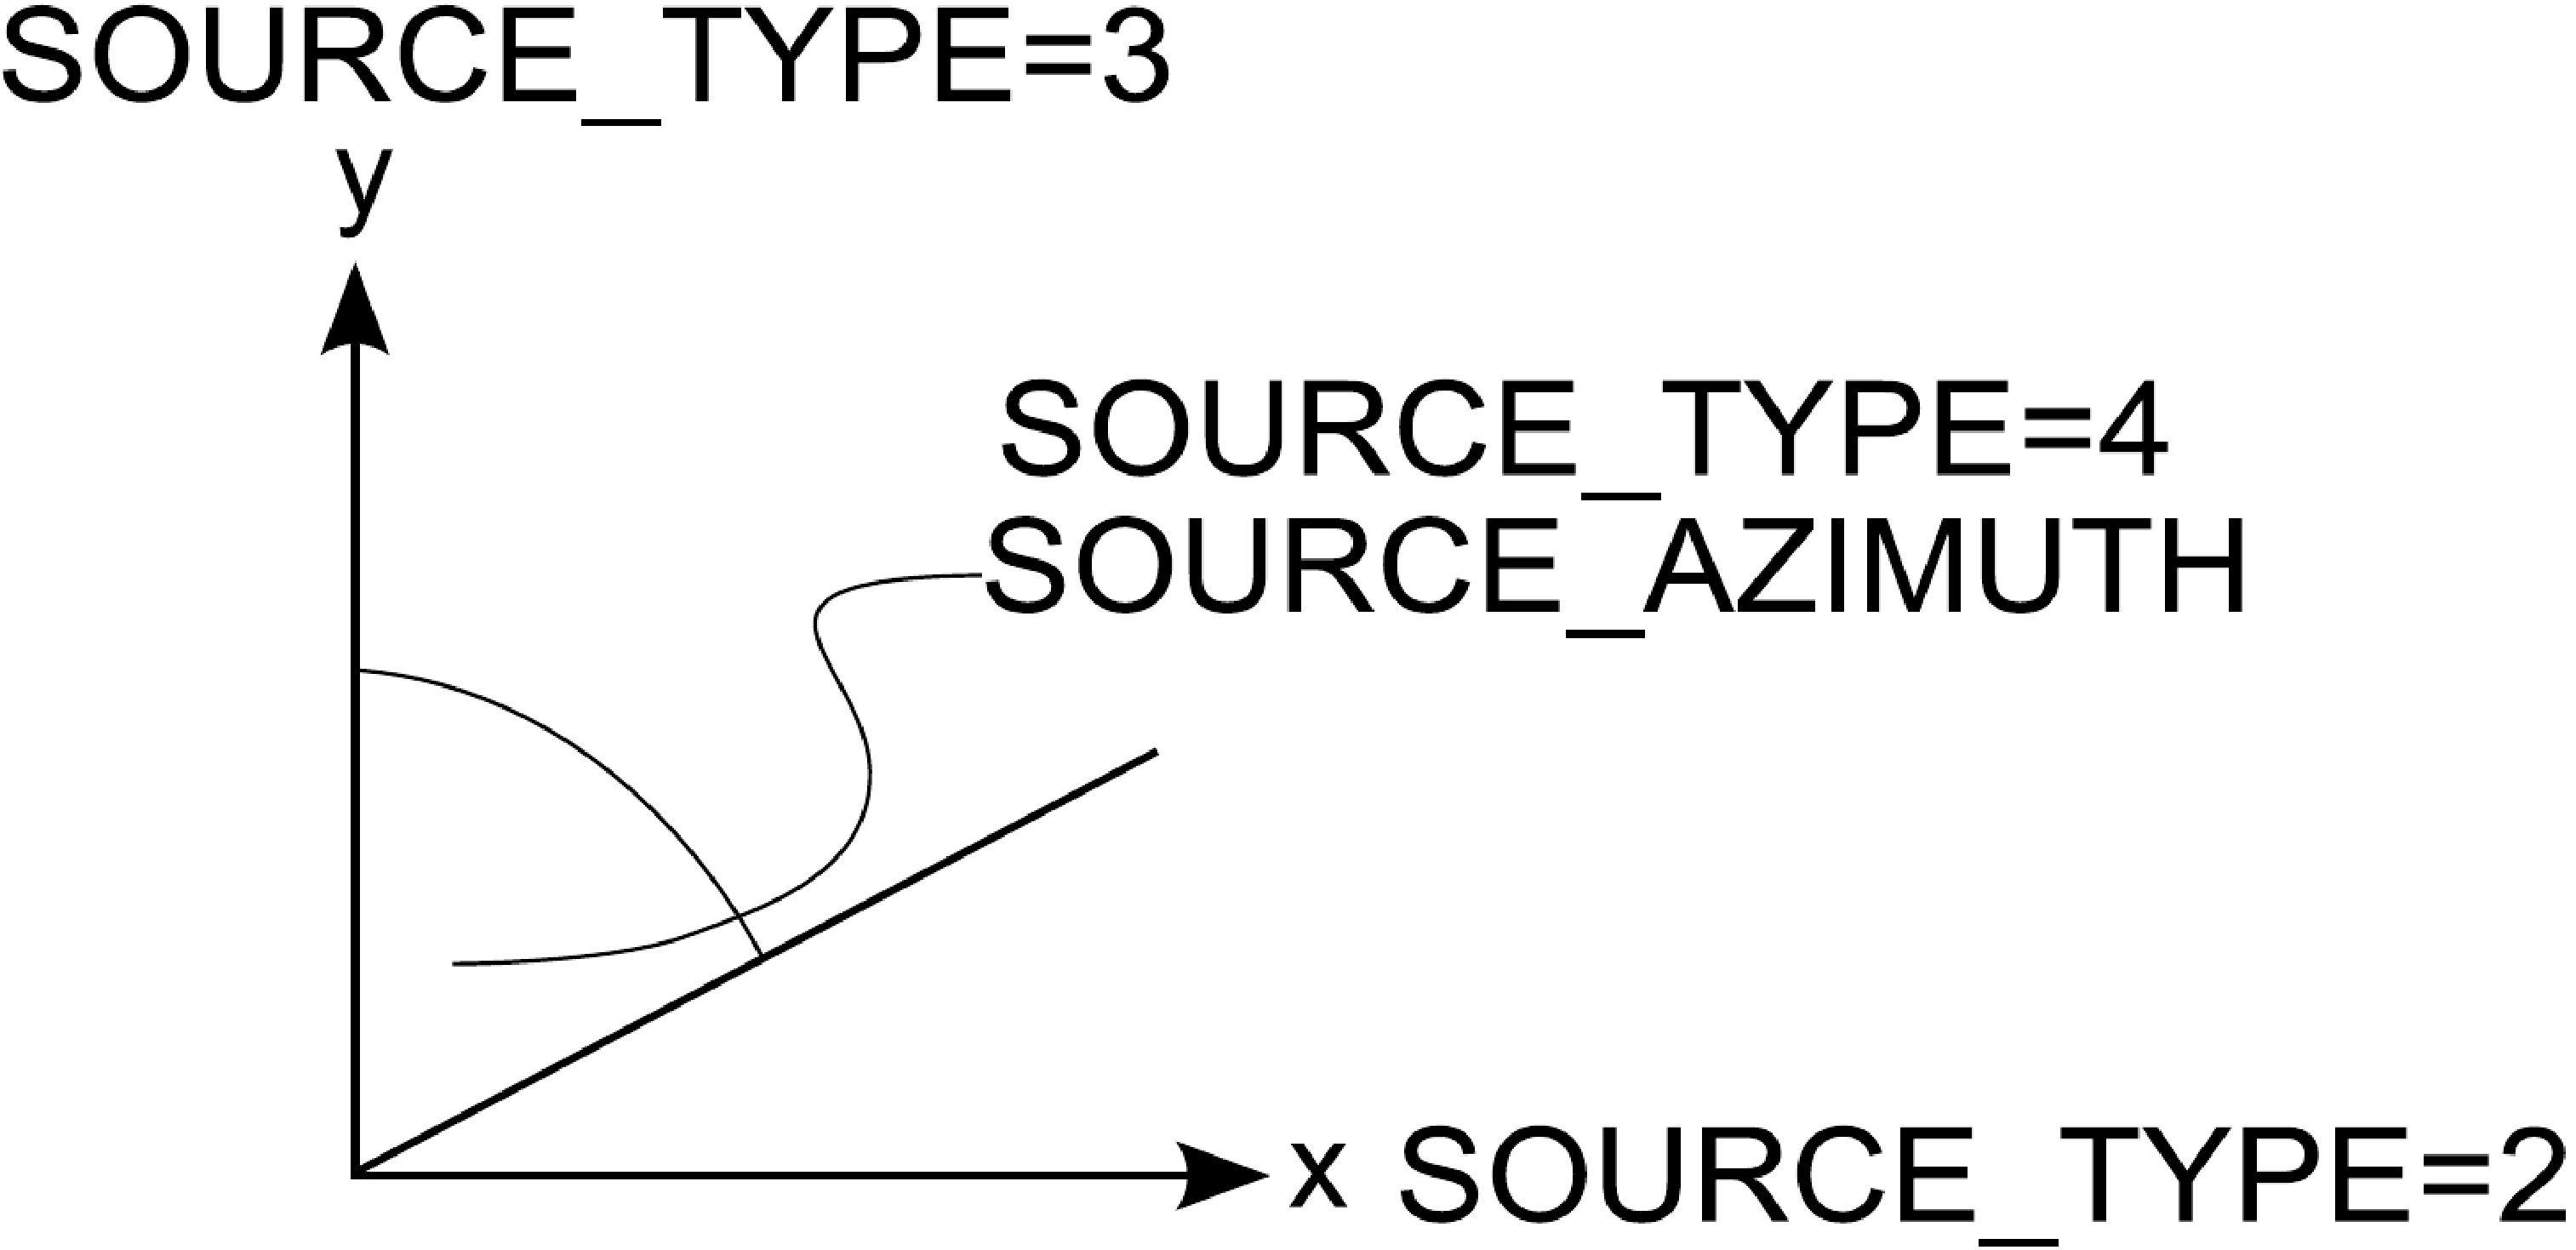
\includegraphics[width=7cm,angle=0]{figures/source_azimuth.pdf}
    \caption{Scheme for \texttt{SOURCE\_TYPE}=4. The parameter \texttt{SOURCE\_AZIMUTH} denotes the angle between the vertical $y$- and horizontal $x$-coordinate.}
    \label{fig_source_azimuth}
\end{figure}

\texttt{SOURCE\_TOPO} : place sources relative to topography (=1) or at absolute depth (=0)

The \texttt{SOURCE\_TOPO} option is only relevant in case sources are read from a file (\texttt{SRCREC}=1). Under normal circumstanes, i.e., when \texttt{SOURCE\_TOPO}=0 which is also the default, sources are placed at the absolute depth specified in the external source file given by \texttt{SOURCE\_FILE}. However, sometimes an explicit air layer is part of the model in case the Earth has topography. When \texttt{SOURCE\_TOPO}=1, then sources are not placed at an absolute depth value but the depth specified in the external source file becomes a depth below topography. The topography is determined by opening the P-wave velocity model and scanning each trace from top to bottom until a change of the first P-wave velocity value that was read in is found (this usually is the interface between air and the solid Earth). The actual P-wave velocity value of the first (air) layer itself does not matter, we only scan for a change. Example: if you would like to simulate sources in 12\;m deep shot holes along a free surface with topographic variations, you need an explicit air layer in the model, you need to set the depth of the source (YSRC, see below) to "12.0" in the external source file, and you finally need to switch on the \texttt{SOURCE\_TOPO} option.

\texttt{SRCREC} : read source positions (from external \texttt{SOURCE\_FILE}=1; from internal \texttt{PLANE\_WAVE}=2)\\
\texttt{SOURCE\_FILE} : external source file name

A source file should have the following format:
\begin{verbatim}
XSRC     YSRC     TD     FC     AMP      SOURCE_AZIMUTH     SOURCE_TYPE
\end{verbatim}

where

\texttt{XSRC} : $x$-coordinate of a source point (in meters)\\
\texttt{YSRC} : $y$-coordinate (depth) of a source point (in meters)\\
\texttt{TD} : time-delay for the source point (in seconds)\\
\texttt{FC} : center frequency of the source signal (in Hz)\\
\texttt{AMP} : maximum amplitude of the source signal

Optional parameters:\\
\texttt{SOURCE\_AZIMUTH} : If \texttt{SOURCE\_TYPE}=4, it represents the angle in degrees between the $y$- and $x$-directions; a \texttt{SOURCE\_AZIMUTH}=0 corresponds to the case \texttt{SOURCE\_TYPE}=3 and \texttt{SOURCE\_AZIMUTH}=90 corresponds to \texttt{SOURCE\_TYPE}=2 (please note that there is a numerical inaccuracy between \texttt{SOURCE\_TYPE}=2 and its analog version \texttt{SOURCE\_AZIMUTH}=90)\\
\texttt{SOURCE\_TYPE} : If \texttt{SOURCE\_TYPE} is set here, the value of \texttt{SOURCE\_TYPE} in the input file is ignored

\texttt{RUN\_MULTIPLE\_SHOTS} : multiple shots (modeled simultaneously=0; modeled individually=1)

This parameter defines if multiple shots are modeled simultaneously or whether each shot is modeled individually. If the parameter is set to 0, multiple sources are modeled together. If more than one source is defined in \texttt{SOURCE\_FILE}, each source is triggered at the same time. For \texttt{RUN\_MULTIPLE\_SHOTS}=1, every source specified in the \texttt{SOURCE\_FILE} is modeled individually. The \texttt{SEIS\_FILE} name then contains the number of the shot, e.g., \texttt{test\_vx.su.shot1.0}.

\texttt{PLANE\_WAVE\_DEPTH} : Depth of plane wave excitation (in meters)\\
\texttt{PLANE\_WAVE\_ANGLE} : Dip of plane wave from vertical (in degrees)

In some applications, e.g., transmission experiments or the simulation of teleseismic events, the generation of plane waves are required. If you specify a \texttt{PLANE\_WAVE\_DEPTH}>0, a plain wave at a depth of \texttt{PLANE\_WAVE\_DEPTH} is excited. In the case of \texttt{PLANE\_WAVE\_DEPTH}<0, point sources are applied; thus, \texttt{SRCREC} should be set to 1, otherwise no sources are applied. The plane wave is simply generated by applying the source time function (\texttt{SOURCE\_SHAPE}) with the source characteristic (\texttt{SOURCE\_TYPE}) at each grid point along a straight line (2D modeling). You can also excite plane waves with a certain dip from the vertical direction. See Fig.~\ref{fig_plane_wave} for a description of the geometry for the generation of dipping plane waves. In case of plane waves, the duration of the source signal, and hence the center frequency of the source (\texttt{1/TS}), is specified by $TS$ in the parameter file. In case of point sources (\texttt{PLANE\_WAVE\_DEPTH}=0.0 and \texttt{SRCREC}=1) the center frequency is defined in \texttt{SOURCE\_FILE} together with the location and the time delay. In case of point sources, the parameter $TS$ is ignored.
\begin{figure}[ht!]
\centering
    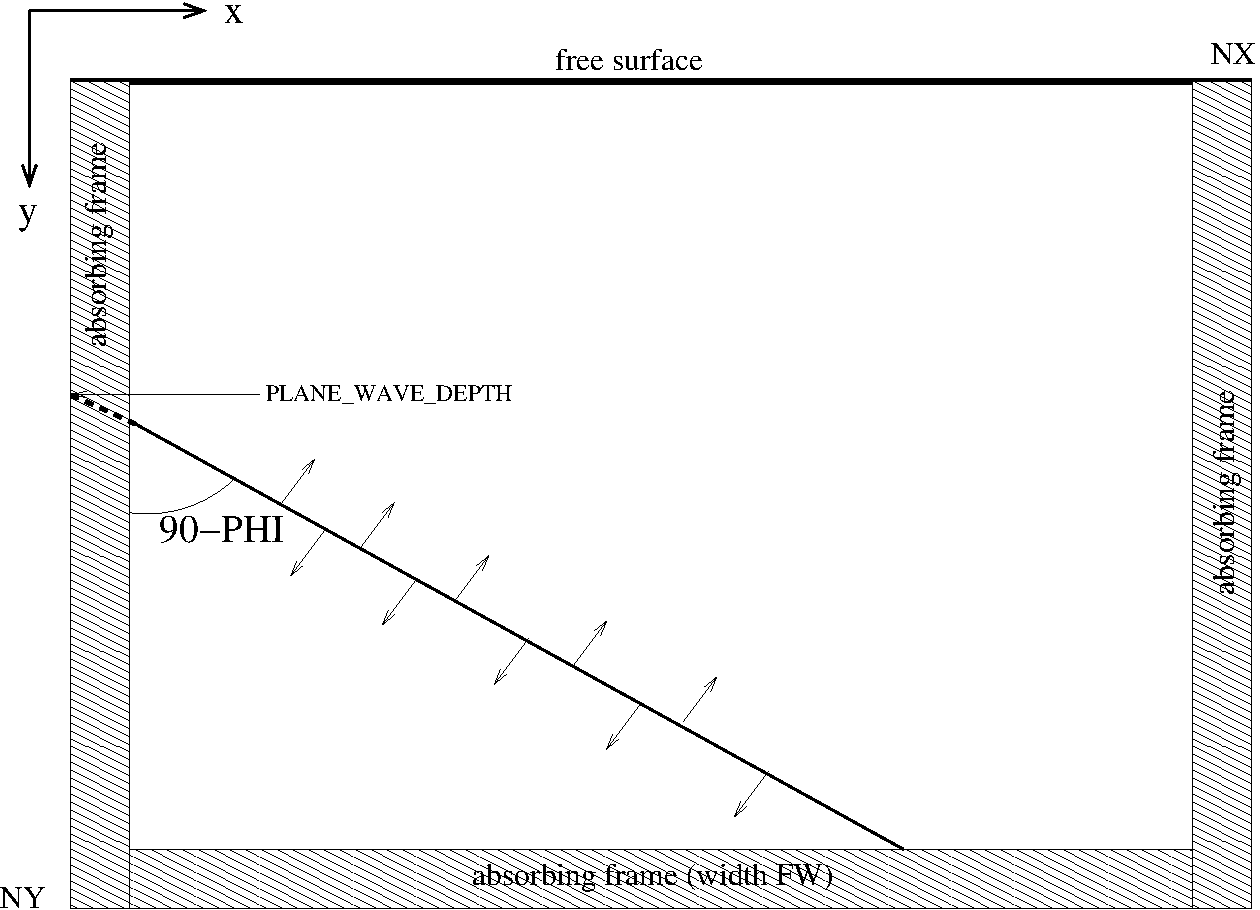
\includegraphics[width=12cm,angle=0]{figures/plane_wave.pdf}
    \caption{Plane waves are generated by assigned source points along  straight lines (2D simulation) or planar planes (3D simulation) with the source wavelet. The parameter \texttt{PLANE\_WAVE\_DEPTH} defines the depth of this line/plane at $x=0$, and the parameter \texttt{PLANE\_WAVE\_ANGLE} specifies the incidence angle with respect to the vertical direction (\texttt{PLANE\_WAVE\_ANGLE}=0 corresponds to vertical incidence).}
    \label{fig_plane_wave}
\end{figure}

\subsection{Generation of models}
\label{gen_of_mod}
\begin{verbatim}
"Model" : "comment",
            "READMOD" : "1",
            "MFILE" : "model/test/TTI_Thomsen_1",
            "WRITE_MODELFILES" : "0",
\end{verbatim}

with

\texttt{READMOD} : read model parameters from \texttt{MFILE} (yes=1; generated \enquote{on the fly}=0)\\
\texttt{MFILE} : basename for the model files, used to read from file and/or to write model for validation\\
\texttt{WRITE\_MODELFILES} : switch on which models are written to file if generated internally \enquote{on the fly} (no model=0; all models=1; only the density model=2).

If \texttt{READMOD}=1, the P-wave, S-wave, and density model grid (if $L=0$, see Chapter~\ref{Q-approximation}) and additionally the attenuation grids (if $L>0$) are read from external files. These files can either be in plain binary format, or SU format -- if SU-formatted files (suffix \texttt{.su}) are present, they will be preferred. Note that the upper left sample of the model (i.e., the first sample on the first trace) is considered to be at Cartesian coordinate $(0,0)$. \texttt{MFILE} defines the basic file name that is expanded by the following extensions: \textbf{P-wave velocity model} \enquote{.vp.su} (or \enquote{.vp}), \textbf{S-wave velocity model} \enquote{.vs.su} (or \enquote{.vs}), both in \SI{}{m/s}, \textbf{density model} \enquote{.rho.su} (or \enquote{.rho}) in \SI{}{kg/m^3}, \textbf{P-wave attenuation model} \enquote{.qp.su} (or \enquote{.qp}), \textbf{S-wave attenuation model} \enquote{.qs.su} (or \enquote{.qs}). In case of anisotropy, the program will also read the \textbf{Thomsen parameter models} \enquote{.epsilon.su} (or \enquote{.epsilon}) and \enquote{.delta.su} (or \enquote{.delta}), and in case of TTI the tilt angle \enquote{.theta.su} (or \enquote{.theta}). The angle is defined as angle in degree against the vertical axis, with positive angles being measured anti-clockwise. A constant zero-degree tilt angle section for TTI corresponds to the VTI case.

In plain binary files, each material parameter value must be saved as 32-bit (4-byte) native float. The fast dimension is the $y$-direction (see, e.g., \texttt{src/readmod*.c}). The number of samples for the entire model in the $x$-direction is $NX$ and the number of values in the $y$-direction is always $NY$. The file size of each model file thus must be $NX*NY*4$ bytes. You may check the model structure using the SU command \textbf{ximage}: \texttt{ximage n1=$<$NY$>$ n2=$<$NX$>$ $<$ model/test.vp}.

For SU-formatted model files, the set-up is similar. They must use 32-bit native floats. The number of samples per trace must equal $NY$, and the number of traces must equal $NX$. Note: if there are more than $NY$ samples per trace in the SU file, the additional samples per trace will be ignored. That means, the code will only ever read $NY$ samples. The same holds if there are more than $NX$ traces in the file -- the code will only ever read $NX$ traces (starting from the beginning of the file) as specified in the parameter file. In case the entire file is used, it should have size $NX*NY*4+NX*240$ bytes (as the SU tracer header has a length of 240 bytes).

If \texttt{READMOD}=0, the model is generated \enquote{on the fly} by SOFI2D, i.e., it is generated internally before the time loop starts. Note that if \texttt{READMOD}=0, the function building the model is called from within the software and must therefore be specified in the Makefile; you need to re-compile SOFI2D by changing to the \texttt{build} directory and typing \texttt{make all} in case you would like to modify and/or update the internal model generation.

As the variable \texttt{MFILE} is also used to write the internally created model(s), you can specify which models are output (\texttt{WRITE\_MODELFILES}). Be aware that the output of additional models besides density will cause extra (but temporal) memory allocation of the size of the local subgrid times the number of models! 
% The actual $V_p$ and $V_s$ models can be easily calculated from the following relationships:
% \begin{subequations}
%     \begin{align}
%         U &= V_s \cdot V_s \cdot rho\;,\\
%         Pi &= V_p \cdot V_p \cdot rho\;.
%         \label{eq_U_PI}
%     \end{align}
% \end{subequations}
    
\subsection{Q-approximation}
\label{Q-approximation}
\begin{verbatim}
"Q-approximation" : "comment",
            "L" : "1",
            "F_REF" : "50.0",
            "FL1" : "50.0", 
            "TAU" : "0.1",
\end{verbatim}

with 

\texttt{L} : number of relaxation mechanisms (elastic=0; viscoelastic>0; up to 5)\\
\texttt{F\_REF} : reference frequency\\
\texttt{FL1} : relaxation frequencies (one for each relaxation mechanism; \texttt{FL2,...,FL5})\\
\texttt{TAU} : ratio of strain-retardation and stress-relaxation times (describes the directional variation of attenuation); only used for internal model generation

These lines are omitted in the elastic version (if \texttt{L}=0). The frequency dependence of the (intrinsic) quality factor $Q(\omega)$ is defined by the \texttt{L} relaxation frequencies (\texttt{FL1}$=f_l=2\pi/\tau_{\sigma l}$). In the current model (see \texttt{model.c}), these values are assigned to all gridpoints for both P- and S-waves. Thus, intrinsic attenuation is homogeneous and equal for P- and S-waves ($Q_p(\omega)=Q_s(\omega)$). However, it is possible to simulate any spatial distribution of absorption by assigning the gridpoints with different $\tau$-values. Note that for a single relaxation mechanism (\texttt{L}=1), $Q \approx 2/\tau$ (\cite{bohlen:02}; $Q(\omega)$ for \texttt{L}=1, \texttt{FL1}$ =f_l=\SI{70}{Hz}$, and \texttt{TAU}$=\tau=0.04$ is shown in Fig. 11). \textcolor{red}{The Matlab script \texttt{/mfiles/qplot.m} can be used to plot $Q(\omega)$ for different values of \texttt{L}, \texttt{FL1}, and \texttt{TAU}}. The script \texttt{qapprox.m} finds optimal values in a way that they fit a desired function $Q(\omega)=$~const in a least-squares sense.

Please note, that due to dispersive media properties the viscoelastic velocity model is only defined for the reference frequency only. In SOFI2D, this reference frequency is specified as the center source frequency. At the exact reference frequency, elastic and viscoelastic models are equivalent. As a consequence, slightly smaller and larger minimum and maximum velocity values occur in the viscoelastic model.

\subsection{Boundary conditions}
\label{abs}
\begin{verbatim}
"Boundary Conditions" : "comment",
            "FREE_SURF" : "0",
            "BOUNDARY" : "0",
            "FW" : "20",
            "ABS_TYPE" : "2",
            "NPOWER" : "4.0",
            "K_MAX_CPML" : "1.0",
            "VPPML" : "3500.0",
            "FPML" : "15.0",
            "DAMPING" : "8.0",
\end{verbatim}

with

\texttt{FREE\_SURF} : free surface at the top of the model (no=0; yes=1)\\
\texttt{BOUNDARY} : periodic boundary condition at edges (no=0; left and right=1)\\ 
\texttt{FW} : width of absorbing frame in grid points (no=0; exponential damping applied at the left/right, front/back, and bottom of the grid>0 - \cite{cerjan:85})\\
\texttt{ABS\_TYPE}: type of absorbing boundary (CPML=1; damping=2)\\
\texttt{NPOWER} : exponent for calculation of damping profile \\
\texttt{K\_MAX\_CPML} : \\
\texttt{VPPML} : attenuation velocity within the PML, approximately the propagation velocity of the dominant wave near the model boundaries (in m/s)\\
\texttt{FPML} : dominant signal frequency (in Hz)

In some cases, it is useful to apply periodic boundary conditions, for example when modeling seismic wave transmission through random media (\cite{bohlen:02}). If \texttt{BOUNDARY}=1 no absorbing boundaries are installed at the left and right sides of the grid. Instead, wavefield information is copied from left to right and vice versa. The effect is, for example, that a wave which leaves the model at the left side enters the model again at the right side.

The convolutional perfectly matched layer (CPML) boundary condition implementation is based on \citet{komatitsch:07} and \citet{martin:09}. A width of the absorbing frame of \texttt{FW}=10-20 grid points should be sufficient. For the optimal realization of the PML boundary condition, you have to specify the dominant signal frequency \texttt{FPML} occurring during the wave simulation; this is usually the center source frequency \texttt{FC} specified in the source file.

\texttt{DAMPING} : attenuation at the edges of the grid (in \%)

With the \texttt{DAMPING} boundary, attenuation is specified at the edges of the numerical grid, i.e., amplitudes are multiplied by a factor of 1-\texttt{DAMPING} at the edges. The width of the absorbing frame should be \texttt{FW}>20 gridpoints (\cite{cerjan:85}); a good choice is 8.0$\%$; for larger values, reflections at the onset of the absorbing frame might occur (\cite{cerjan:85}). In order to avoid such an impedance contrast between the model domain and the absorbing boundary layer, \texttt{FW} should increase and \texttt{DAMPING} should decrease. If \texttt{FREE\_SURF}=0, damping is also applied at the top of the model.

\subsection{Wavefield snapshots}
\begin{verbatim}
"Snapshots" : "comment",
            "SNAP" : "1",
            "TSNAP1" : "0.01",
            "TSNAP2" : "0.5",
            "TSNAPINC" : "0.01",
            "IDX" : "1",
            "IDY" : "1",
            "SNAP_FORMAT" : "3",
            "SNAP_FILE" : "./snap/hh_e_t",
\end{verbatim}

with

\texttt{SNAP} : output of snapshots (no seismograms=0; particle velocities=1; pressure field/hydrophones=2; curl and divergence energy=3; velocities, pressure, and energy=4)\\
\texttt{TSNAP1} : first snapshot (in seconds)\\
\texttt{TSNAP2} : last snapshot (in seconds)\\
\texttt{TSNAPINC} : increment (in seconds; should be a multiple of \texttt{DT})\\
\texttt{IDX} : increment in $x$-direction (grid points)\\
\texttt{IDY} : increment in $y$-direction (grid points)\\
\texttt{SNAP\_FORMAT} : data format (ASCII=2; binary=3)\\
\texttt{SNAP\_FILE} : output basename

If \texttt{SNAP}>0, wavefield information (particle velocities, pressure or curl and divergence of particle velocities) for the entire model is saved on disk; therefore, be sure that you have enough free space! Each PE is writing its sub-volume to disk. The filenames have the basename \texttt{SNAP\_FILE} plus an extension that indicates the PE number in the logical processor array (see Fig.~\ref{fig_grid}). Note that the file sizes increase during the simulation. It may therefore be necessary to reduce the amount of snapshot data by increasing \texttt{IDX} and \texttt{IDY} and/or \texttt{TSNAPINC}. In order to merge the separate snapshot of each PE after the completion of the wave modeling, you can use the program \texttt{snapmerge}.

\subsection{Receivers}
\begin{verbatim}
"Receiver" : "comment",
            "SEISMO" : "0",
            "READREC" : "1",
            "REC_TOPO" : "0",
            "REC_FILE" : "./receiver/receiver.dat",
            "REFRECX, REFRECY" : "0.0 , 0.0",
            "XREC1,YREC1" : "50.0 , 1.0",
            "XREC2,YREC2" : "350.0 , 1.0",
            "NGEOPH" : "1",
\end{verbatim}

with

\texttt{SEISMO} : output of seismograms (no seismograms=0; particle velocities=1; pressure/hydrophones=2; curl and div=3; everything=4)

If \texttt{SEISMO}>0, seismograms are saved on disk; when \texttt{SEISMO} is 1, $x$- and $y$-components of particle velocity will be written according to parameters specified in section~\ref{seismograms}; if \texttt{SEISMO}=2, pressure (sum of the diagonal components of the stress tensor) recorded at the receiver locations is written; if SEISMO=3 the curl and divergence are saved. The curl and divergence of the particle velocities are useful to separate P- and S-waves in the snapshots of the wavefield. SOFI2D calculates the divergence and the magnitude of the curl of the particle velocity field (\cite{dougherty:88}). The motivation for this is as follows: according to \citet{morse:53}, the energy of P- and S-wave particle velocities, respectively, are
\begin{equation}
    E_p=\left(\lambda + 2 \mu\right) \left[ \text{div}(\vec{v}) \right]^2 \quad \mbox{and} \quad E_s=\mu \left|\text{rot}(\vec{v})\right|^2\;,
    \label{eq_E}
\end{equation}
where $\lambda$ and $\mu$ are the Lam\`{e} parameters, and $\vec{v}$ is the particle velocity vector. In order to preserve the divergence and curl sign information  while showing relative compressional and shear particle velocity amplitudes, we plot the following quantities:
\begin{equation}
    \bar{E}_p = \text{sign}(\text{div}\,\vec{v}) E_p^{1/2} \quad \mbox{and} \quad \bar{E}_s= \text{sign}(\text{rot}\,\vec{v}) E_s^{1/2}\;.
    \label{eq_e}
\end{equation}
The magnitudes of $\bar{E}_p$ and $\bar{E}_s$ are proportional to the magnitudes of the P- and S-particle velocities, respectively. Note that interface waves like Rayleigh waves contain both a P- and S-wave component and therefore show up on both quantities of Eq.~\ref{eq_e}.

\texttt{READREC} : read receiver positions from file (from the parameter file=0; from an external file=1)

\texttt{REC\_TOPO} : place receivers relative to topography (=1) or at absolute depth (=0)

The \texttt{REC\_TOPO} option is only relevant in case receivers are read from an external file (\texttt{READREC}=1). Under normal circumstanes, i.e., when \texttt{REC\_TOPO}=0 which is also the default, receivers are placed at the absolute depth specified in the external receiver file given by \texttt{REC\_FILE}. However, sometimes an explicit air layer is part of the model in case the Earth has topography. When \texttt{REC\_TOPO}=1, then receivers are not placed at an absolute depth value but the depth specified in the external receiver file becomes a depth below topography. For details on how the topography is found, please check the \texttt{SOURCE\_TOPO} option.

\texttt{REC\_FILE} : external receiver file name (ASCII-file)\\
\texttt{REFREC} : reference point for receiver coordinate system (if 1, the following 3 parameters are ignored)\\
\texttt{XREC1,YREC1} : position of the first receiver (in meters) \\
\texttt{XREC2,YREC2} : position of the last receiver (in meters)\\
\texttt{NGEOPH} : distance between two adjacent receivers (in grid points)

The locations of the receivers may either be specified in the parameter file or in a separate file (\texttt{REC\_FILE}). When reading them from the parameter file, it is assumed that the receivers are located along a straight line. The first receiver position is defined by (\texttt{XREC1}, \texttt{YREC1}), and the last receiver position by (\texttt{XREC2}, \texttt{YREC2}). The spacing between receivers is \texttt{NGEOPH} grid points; a vertical seismic profile (VSP) is realized when \texttt{XREC1=XREC2} and \texttt{YREC1<YREC2}. When reading from an ASCII-file, each line should contain the receivers coordinates (in meters) as below: the horizontal $x$- and then the vertical $y$-coordinate of each receiver position, respectively.
\begin{verbatim}
50.0   2.0
100.0  2.0
150.0  2.0
...
\end{verbatim}

These receiver coordinates are possibly shifted by \texttt{REFREC}[1] and \texttt{REFREC}[2] into the $x$- and $y$-direction, respectively. This allows for completely moving the receiver spread without modifying \texttt{REC\_FILE}. This may be useful for the simulation of moving profiles in reflection seismics.

Receivers are always located on full grid indices, i.e., a receiver that is located between two grid points will be shifted by the FD program to the closest next grid point. It is not possible to output seismograms for arbitrary receiver locations since this would require a certain wavefield interpolation. It is important to note that the actual receiver positions defined in the \texttt{REC\_FILE} or in \texttt{sofi2D.json} may vary by $DH/2$ due to the staggered positions of the particle velocities and stress tensor components.

\subsection{Receiver array}
\begin{verbatim}
"Receiver array" : "comment",
            "REC_ARRAY" : "0",
            "REC_ARRAY_DEPTH" : "70.0",
            "REC_ARRAY_DIST" : "40.0", 
            "DRX" : "4",
\end{verbatim}

with

\texttt{REC\_ARRAY} : number of receivers in 1D receiver array (no simulation=0)\\
\texttt{REC\_ARRAY\_DEPTH} : depth of first plane (in meters)\\
\texttt{REC\_ARRAY\_DIST} : increment between receiver planes (in meters)\\
\texttt{DRX} : increment between receivers in each plane (in gridpoints)

A horizontal 1D array of receivers is simulated if \texttt{REC\_ARRAY}>0. This option specifies the number of receiver planes horizontal to the surface of the model (parallel to the $x$-axis). The distance between receivers within each plane is \texttt{DRX*DH} (in meters).

\subsection{Seismograms}
\label{seismograms}
\begin{verbatim}
"Seismograms" : "comment",
            "NDT" : "5",
            "SEIS_FORMAT" : "1",
            "SEIS_FILE" : "./su/test_t003",
\end{verbatim}

with

\texttt{NDT} : sampling rate (in FD time steps)

If \texttt{SEISMO}>0, seismograms recorded at the receiver positions are written to the corresponding output files. The sampling rate of the seismograms is \texttt{NDT*DT} seconds. In case of a small time step interval and a large number of time steps, it might be useful to choose a relatively large \texttt{NDT} to avoid an unnecessary detailed sampling of the seismograms and consequently large files of seismogram data.

\texttt{SEIS\_FORMAT} : data output format (SU=1; ASCII=2; binary=3)

It is recommended to use SU (native 4-byte-floats (IEEE on PC)/little endian on PC) format for saving the seismograms. The main advantage of this format is that the time step interval (\texttt{NDT*DT}) and the acquisition geometry (shot and receiver locations) are stored in the corresponding SU header words. Moreover, additional header words like offset are set by SOFI2D. This format thus facilitates a further visualization and processing of the synthetic seismograms. Note, however, that SU cannot handle sampling rates smaller than \SI{1.0e-3}{ms} and the number of samples is limited to about \SI{32000}{}. In such cases, you should increase the sampling rate by increasing \texttt{NDT}. If this is impossible (for example, because the Nyquist criterion is violated), you must choose a different output format (ASCII or binary). 

SU-files can be merged together using the Unix command \texttt{cat}. 

\texttt{SEIS\_FILE} : basename for output of seismograms (\texttt{SEISMO})

Separate seismogram files are output, looking like \texttt{SEIS\_FILE\_vz.su} or \texttt{SEIS\_FILE\_div.bin}. Each PE internally stores seismograms which are recorded in its portion of the grid. After finishing the time step loop, the seismogram parts are internally exchanged and the merged seismograms are collectively saved to the output file. A certain suffix is added to the basename \texttt{SEIS\_FILE} dependent on the chosen \texttt{SEISMO} option (pressure, particle velocity, curl, and divergence). To give an example, the program writes the merged seismograms of the $x$-component of particle velocity to \texttt{SEIS\_FILE\_vx.su}.

\textbf{Wavelet shapes -- practical issues}\\
When using an explosive source, a pressure sensor, and a Ricker wavelet as source function with the standard elastic wave equation, the resulting seismograms have to be integrated one-and-a-half times (\texttt{sufrac power=-1.5}) in order to get back to the original Ricker shape and its spectrum. In addition, there is a polarity reversal due to the definition of pressure; in such a case, the additional parameter \texttt{phasefac=1} would revert the polarity. When using a force source, a velocity sensor, and a Ricker wavelet as source function with the standard elastic wave equation, the resulting seismograms have to be half-integrated (\texttt{sufrac power=-0.5}) in order to get back to the original Ricker shape and its spectrum. There is no polarity reversal.

\subsection{Monitoring the simulation}
\begin{verbatim}
"Monitoring the simulation" : "comment",
            "LOG_FILE" : "log/test.log",
            "LOG" : "0",
            "LOG_VERBOSITY" : "INFO",
            "OUT_TIMESTEP_INFO" : "100",
\end{verbatim}

with

\texttt{LOG\_FILE} : log-file for information about progress of program (each PE is printing log-information to \texttt{LOG\_FILE.MYID})\\
\texttt{LOG} : output of logging information of node (all ranks output to terminal=0; all ranks output to \texttt{LOG\_FILE}=1; rank 0 outputs to terminal and all other ranks to \texttt{LOG\_FILE}=2)

SOFI2D can output a lot of useful and debug information about the modeling parameters and the status of the modeling process. The major part of this information is output by the main MPI process. The \texttt{LOG} parameter in the \texttt{json} file sets the logging output stream. If \texttt{LOG}=0, the main MPI process writes its log to \texttt{stdout}, i.e., on the terminal; this is generally recommended  to monitor the modeling process. You may want to save this screen log to an output file by adding \texttt{2>\&1 | tee sofi2D.jout} to your start command (if you use a queuing system, this output is normally captured anyway and returned by the queuing system at the end of the job). \texttt{LOG}=1 sends all output to log files as specified in the \texttt{json} file. \texttt{LOG}=2 send the output of the main MPI process to \texttt{stdout} and all other ranks write their output to log files.\\

\texttt{LOG\_VERBOSITY} : set how much information is output (\texttt{DEBUG}, \texttt{INFO}, \texttt{WARN}, \texttt{SILENT})

If the parameter is not given, \texttt{LOG\_VERBOSITY} is internally set to \texttt{INFO}, which means the program should output information that is useful for the user. On \texttt{DEBUG} level, additional output (including code line numbers) occurs which can help in debugging issues. On level \texttt{WARN}, only warnings and errors are output, while \texttt{SILENT} means only errors are output -- they cannot be ignored by the user.

\texttt{OUT\_TIMESTEP\_INFO} : time step increment upon which information is output

As the output of information can both slow down the computation for very small models and produce very large log files, you can choose by \texttt{OUT\_TIMESTEP\_INFO} after how many time steps such intermediate information is logged.

% {\subsection{\enquote{On the fly} definition of material parameters}}
% \label{model_def_func}
% If you choose to create the model \enquote{on the fly}, the distribution of the material parameters P-wave velocity $v_p$, S-wave velocity $v_s$, and density $\rho$ for the simple block model has to be defined in the function \texttt{hh\_elastic.c} that can be found in the \texttt{src} folder.

% \begin{verbatim}
% /* -------------------------------------------------------------
%  *   Model homogeneous half space
%  *   if variable "h" is decreased, a layer over half-space is gained
%  *   ------------------------------------------------------------- */

% #include "fd.h"

% void model_elastic(float  **  rho, float **  pi, float **  u){

% 	/*--------------------------------------------------------------------------*/
% 	/* extern variables */

% 	extern int NX, NY, NXG, NYG,  POS[3], MYID;
% 	extern int WRITE_MODELFILES;
% 	extern float DH;
% 	extern char  MFILE[STRING_SIZE];	

% 	/* local variables */
% 	float muv, piv, Vp, Vs, Rhov;
% 	float y;
% 	int i, j, ii, jj;
% 	char modfile[STRING_SIZE];
% 	float ** pwavemod=NULL, ** swavemod=NULL;


% 	/*-----------------material property definition -------------------------*/	

% 	/* parameters for layer 1 */
% 	const float vp1=3500.0, vs1=2000.0, rho1=2000.0, h=100000.0;


% 	/* parameters for layer 2 */
% 	const float vp2=5400.0, vs2=3700.0, rho2=2500.0;


% 	/*-----------------------------------------------------------------------*/

% 	if (WRITE_MODELFILES==1) {
% 		pwavemod  =  matrix(0,NY+1,0,NX+1);
% 		swavemod  =  matrix(0,NY+1,0,NX+1);
% 	}

% 	/* loop over global grid */
% 	for (i=1;i<=NXG;i++){
% 		for (j=1;j<=NYG;j++){

% 			/* calculate coordinate in m */
% 			y=(float)j*DH;

% 			/* two layer case */
% 			if (y<=h){
% 				Vp=vp1; Vs=vs1; Rhov=rho1; }


% 			else{
% 				Vp=vp2; Vs=vs2; Rhov=rho2; }

% 			/* homogenous case */
% 			// 				vp=vp1; vs=vs1; rhov=rho1;

% 			muv=Vs*Vs*Rhov;
% 			piv=Vp*Vp*Rhov;

% 			/* only the PE which belongs to the current global gridpoint
% 				  is saving model parameters in his local arrays */
% 			if ((POS[1]==((i-1)/NX)) &&
% 					(POS[2]==((j-1)/NY))){
% 				ii=i-POS[1]*NX;
% 				jj=j-POS[2]*NY;

% 				u[jj][ii]=muv;
% 				rho[jj][ii]=Rhov;
% 				pi[jj][ii]=piv;
% 				if (WRITE_MODELFILES==1)
% 				{
% 					pwavemod[jj][ii]=Vp;
% 					swavemod[jj][ii]=Vs;
% 				}
% 			}
% 		}
% 	}

% 	/* each PE writes his model to disk */

% 	/* only the density model is written to file */
% 	if (WRITE_MODELFILES==2) {
% 		sprintf(modfile,"%s.SOFI2D.rho",MFILE);
% 		writemod(modfile,rho,3);
% 		MPI_Barrier(MPI_COMM_WORLD);
% 		if (MYID==0) mergemod(modfile,3);
% 	}

% 	/* all models are written to file */
% 	if (WRITE_MODELFILES==1) {
% 		sprintf(modfile,"%s.SOFI2D.u",MFILE);
% 		writemod(modfile,u,3);
% 		MPI_Barrier(MPI_COMM_WORLD);
% 		if (MYID==0) mergemod(modfile,3);

% 		sprintf(modfile,"%s.SOFI2D.pi",MFILE);
% 		writemod(modfile,pi,3);
% 		MPI_Barrier(MPI_COMM_WORLD);
% 		if (MYID==0) mergemod(modfile,3);

% 		sprintf(modfile,"%s.SOFI2D.vp",MFILE);
% 		writemod(modfile,pwavemod,3);
% 		MPI_Barrier(MPI_COMM_WORLD);
% 		if (MYID==0) mergemod(modfile,3);

% 		sprintf(modfile,"%s.SOFI2D.vs",MFILE);
% 		writemod(modfile,swavemod,3);
% 		MPI_Barrier(MPI_COMM_WORLD);
% 		if (MYID==0) mergemod(modfile,3);

% 		sprintf(modfile,"%s.SOFI2D.rho",MFILE);
% 		writemod(modfile,rho,3);
% 		MPI_Barrier(MPI_COMM_WORLD);
% 		if (MYID==0) mergemod(modfile,3);
% 	}


% 	if (WRITE_MODELFILES==1) {
% 		free_matrix(pwavemod,0,NY+1,0,NX+1);
% 		free_matrix(swavemod,0,NY+1,0,NX+1);
% 	}
% }
% \end{verbatim}

% As you can see from lines
% \begin{verbatim}
% 	sprintf(modfile,"%s.mod",MFILE);
% 	writemod(modfile,rho,3);
% \end{verbatim}
% the density model is written to file to be displayed as described in Chapter~\ref{gen_of_mod}. As a base name for the model file, the variable \texttt{MFILE} from the input file is used that actually specifies the external velocity and density files. \textcolor{red}{Note, that the thickness of the first layer \textit{h} is set to \si{10}{km}, which is larger than the vertical extension (\texttt{NY*DH}=\SI{5400}{m}). In this way, we effectively created a homogeneous model while demonstrating a two-layer case. Simple decrease the variable \textit{h} to \SI{2700}{} and a real two-layer model is created. Generally, you only have to modify the material property definitions in the upper part of the model file and code some if statements to construct simple structures such as planes, cubes, tubes, etc.}

% \textcolor{red}{\subsection{Compilation of \texttt{sofi2D}}}
% \label{compexec}
% The source codes are located in the directory \texttt{src}. To compile SOFI2D, the name of the model function has to be entered in the \texttt{MAKEFILE}. Depending on your MPI environment (MPI distribution), you may need to modify the compiler options in \texttt{src/Makefile}. For a few typical platforms, the compiler options are available in \texttt{src/Makefile}. It is often useful to enable the highest level of optimization (typically -03 or -04). 
% \begin{verbatim}
% # Makefile for SOFI2D

% #--------------------------------------------------------
% # edit here:

% # source code for model generation
% # model file for viscoelastic modeling L>0
% MODEL_V = hh_visco.c
% # model file for elastic modeling L=0
% MODEL_E = hh_elastic.c
% # model file for viscoelastic modeling (overnight built)
% MODEL_BV = benchmod.c
% # model file for elastic modeling L=0 (overnight built)
% MODEL_BE = benchmod_el.c
% EXEC= ../bin

% EXEC= ../bin

% # Compiler (LAM: CC=hcc, CRAY T3E: CC=cc)

% # ON Linux cluster running LAM
% #CC=hcc
% #LFLAGS=-lm -lmpi 
% #CFLAGS=-Wall -O4

% # ON Linux cluster running OpenMPI and ON MAC
% CC=mpicc
% LFLAGS=-lm -lmpi 
% CFLAGS=-Wall -O3 

% # On CRAY T3E
% # CC=cc

% # On SCHARnet system
% #CC=mpicc
% #LFLAGS=-lm  

% # On HLRN system
% #CC=mpcc
% #LFLAGS=-lm  

% # ALTIX
% #CC=icc
% #CFLAGS=-mp -O3 -ip0
% #LFLAGS=-lmpi -lm 

% # after this line, no further editing should be necessary
% # --------------------------------------------------------
% \end{verbatim}

% To compile the program \texttt{sofi2D}, you must change to the \texttt{src} directory and execute:
% \texttt{make all}  
% or
% \texttt{make sofi2D}  
% The program \texttt{snapmerge} that is used to merge the snapshots (see below) can be compiled with \texttt{make snapmerge}. Since this is not a MPI program (no MPI functions are called), the MPI libraries are not required and any standard compiler (like gcc and cc) can be used to compile this program. The executables \texttt{sofi2D} and \texttt{snapmerge} are located the \texttt{bin} directory.

% \subsection{Running the program}
% \label{compexec1} 
% Each \texttt{sofi2D} run reads the required parameters from a parameter file. An example parameter file was defined in section \ref{modelgeom} \texttt{par/in\_and\_out/sofi2D.json}. The command to start a simulation on 4 processosr with the lowest priority of -19 (in order to allow working on the a workstation while running a simulation) is as follows (please note that we assume you have navigated to the folder \texttt{sofi2D/par}):

% \texttt{mpirun -np 8 nice -19 ../bin/sofi2D ./in\_and\_out/sofi2D.json }

% If you use LAMMPI, the command \texttt{lamboot -v lamhost} must be executed on node 0 which is the PE where \texttt{./par/lamhosts} is the file containing IP addresses of all computing nodes. It is often useful to save the standard output of the program for later reference. The screen output may be saved to \texttt{sofi2D.jout} using 

% \texttt{mpirun -np 8 nice -19 ../bin/sofi2D ./in\_and\_out/sofi2D.json > ./in\_and\_out/sofi2D.jout}

% Combining both the screen and the file output you can execute the following line (this is used in the shell script \texttt{startSOFI2D.sh})

% \texttt{mpirun -np 8 nice -19 ../bin/sofi2D ./in\_and\_out/sofi2D.json | tee \\
% ./in\_and\_out/sofi2D.jout}

% \textcolor{red}{After the output of geometry and model parameters, the code starts the time stepping and displaying timing information:}

% \begin{verbatim} 

%  **************************************************
%  *********** STARTING TIME STEPPING ***************
%  **************************************************

%  real time before starting time loop: 0.00 s.
%  Message from function wavelet written by PE 0
%  1 source positions located in subdomain of PE 0
%  have been assigned with a source signal.

%  Computing timestep 1 of 625

%  **Message from update_v (printed by PE 0):
%  Updating particle velocities ... finished (real time: 0.000 s).
%  particle velocity exchange between PEs ... finished (real time: 0.000 s).

%  **Message from update_s (printed by PE 0):
%  Updating stress components ... finished (real time: 0.000 s).
%  stress exchange between PEs ... finished (real time: 0.000 s).

%  PE 0 is writing snapshot-data at T=0.008000s to
% ./snap/test.bin.vx.00
% ./snap/test.bin.vy.00
% ./snap/test.bin.p.00

% ./snap/test.bin.div.00
% ./snap/test.bin.curl.00

%  total real time for timestep 1 : 0.002 s.

%  Computing timestep 11 of 625

%  **Message from update_v (printed by PE 0):
%  Updating particle velocities ... finished (real time: 0.000 s).
%  particle velocity exchange between PEs ... finished (real time: 0.000 s).

%  **Message from update_s (printed by PE 0):
%  Updating stress components ... finished (real time: 0.002 s).
%  stress exchange between PEs ... finished (real time: 0.000 s).
%  total real time for timestep 11 : 0.003 s.
% \end{verbatim}

% After some waiting time - depending on the model problem and computer performance - we finally get the message:

% \begin{verbatim}
%  Computing timestep 621 of 625

%  **Message from update_v (printed by PE 0):
%  Updating particle velocities ... finished (real time: 0.000 s).
%  particle velocity exchange between PEs ... finished (real time: 0.000 s).

%  **Message from update_s (printed by PE 0):
%  Updating stress components ... finished (real time: 0.000 s).
%  stress exchange between PEs ... finished (real time: 0.000 s).
%  total real time for timestep 621 : 0.000 s.

%  *********** Finish TIME STEPPING ****************
%  **************************************************

%  PE 0 is writing 100 merged seismogram traces (vx)   to  ./su/test_vx.su
%  PE 0 is writing 100 merged seismogram traces (vy)   to  ./su/test_vy.su
%  PE 0 is writing 100 merged seismogram traces (p)    to  ./su/test_p.su
%  PE 0 is writing 100 merged seismogram traces (div)  to  ./su/test_div.su
%  PE 0 is writing 100 merged seismogram traces (curl) to  ./su/test_curl.su

%  **Info from main (written by PE 0):
%  Average times for
%    velocity update:      0.000011 seconds
%    stress update:        0.000014 seconds
%    velocity exchange:    0.000019 seconds
%    stress exchange:      0.000020 seconds
%    timestep:             0.000081 seconds

%  CPU time of program per PE: 0 seconds.
%  Total real time of program: 0.307 seconds.

%  ******************************************************
%  **************** SOFI2D has finished *****************
%  ******************************************************
% \end{verbatim}  

\subsection{Postprocessing}
The wavefield snapshots can be merged using the program \texttt{snapmerge}. The program \texttt{snapmerge} is not an MPI program. Therefore, it can be executed without MPI and the \texttt{mpirun} command. You can run \texttt{snapmerge} on any PC since a MPI environment (e.g., LAM) is not required. You may therefore copy the snapshot outputs of the different nodes to another non-MPI computer to merge the files together. \texttt{snapmerge} reads the required information from the \texttt{sofi2D} parameter file. Simply type

\texttt{../bin/snapmerge /path/to/sofi2D.json}

Depending on the model size and number of MPI processes, the merge process may take some time. For the simple block model, it only takes a few seconds. At the end of the merge process, \texttt{snapmerge} will output SU commands that allow you to run the snapshots as movie.

% The output should read like this:
% \begin{verbatim}
%  x-component of particle velocity (files: ./snap/test.bin.x.??? ).

%  writing merged snapshot file to  ./snap/test.bin.x
%  Opening snapshot files: ./snap/test.bin.x.???  ... finished.
%  Copying... ... finished.
%  Use
%  xmovie n1=100 n2=100  < ./snap/test.bin.x loop=1 label1=Y label2=X title=%g 
%     d1=54.000000 d2=54.000000 f1=54.000000 f2=54.000000 clip=2.332155e-09
%  to play the movie
% \end{verbatim} 